\chapter{Introduction} 
\label{chapter-intro} 

\section{Aim and significance}
This capstone project builds on a long line of research aiming to develop more accurate mathematical and computational models of the visual system. There has recently been evidence suggesting that feed-forward neural networks such as Convolutional Neural Networks (CNNs) turn out to be inaccurate models for the primary visual cortex (V1), even though CNN was initially inspired by the earliest computational model of the primary visual cortex (the Neocognitron model) and has performed well on most computer vision tasks. 
    \begin{figure}[H]
            \centering
                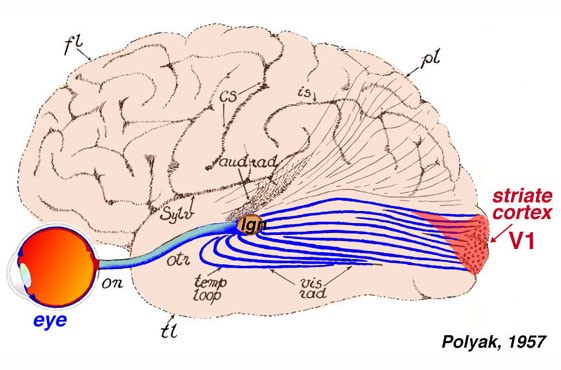
\includegraphics[width=0.25
             \textwidth]{presentation/figures-models/v1.jpg}
                \caption{Visual input goes from the eye to primary visual cortex (V1). Adapted from Polyak (1957).}
            \end{figure} 
            
The central question we will be investigating in this project is the following: how is the structure of artificial neural networks (ANNs) related to that of neurobiological networks in the primary visual cortex? This remains an open question.
    
\par One challenge of comparing the neural network structures is that the neural responses (from both V1 and ANNs) are usually encoded in high-dimensional representation.  Our approach to this question is to infer a neural manifold using dimensionality reduction methods on the neural responses. Informally, the neural manifold shows the clusters of neurons grouped by their firing patterns in response to a given visual stimulus.  This manifold structure implies a functional network (represented by the discrete data graph underlying the continuous manifold) and thus reflects both the neural circuit connections and the neuron’s role in those circuits. 

\par We then compare the neural manifolds in biological and artificial neural networks. For the latter, we will be investigating Convolutinoal Neural Networks (CNNs), Recurrent Neural Networks (RNNs) and the latest Transformer and Perceiver networks. By comparing the manifold structures of biological and artificial neural networks we can make precise inferences about similarities and differences in their respective functional circuits.
  
\par The significance of achieving the goals outlined above is twofold. First, there is significant interest in comparing the structure of artificial and biological neural networks. Artificial neural networks have proved capable of many computer vision tasks at a level competitive to biological systems. However, whether artificial and biological neural networks have the same functional circuit remains an open question. (\cite{Gwilliams221630}) 

\par Second, modeling the visual system is an important task. In the field of neuroscience, despite decades of research, we have not fully understood the science behind visual perception. In the field of AI, more sophisticated models of the visual system could inspire new computational algorithms in solving increasingly demanding computer vision tasks. In fact, research in computer vision has taken many inspirations from neuroscience. In LeCun, Bengio, \& Hinton's seminal work on deep learning (\cite{lecun_deep_2015}), they stated that ``ConvNets have their roots in the Neocognitron," which was one of the earliest computational models of the visual system. 

\section{Historical context}

\par The earliest efforts in modeling the visual system began with Hubel and Wiesel's hierarchy model in the 1960s. Sine then, numerous alternative models were proposed, such as the parallel models and recurrent models, all of which aimed to more accurately reflect the actual neural connectivity in the visual system. 

\subsection{Hierarchy Models}
\par Hubel and Wiesel's hierarchy model (\cite{hubel_receptive_1962}) was the first seminal work on modeling the visual system, which classified the neurons in the primary visual cortex (V1) into simple cells and complex cells. The essential difference between the simple cells and complex cells is that the responses of simple cells are modulated by the spatial phase of a sine grating, whereas the responses of complex cells are largely phase invariant. In other words, as we progress from simple cells to complex cells, the neurons become selective for increasingly complex stimuli and at the same time become more tolerant to the exact position within their receptive fields. 

\par Based on this, a natural way to construct complex cells is to group responses from simple cells with the same orientation preference, but with different phase preferences.

\par This idea directly inspired the Neocognitron model (\cite{fukushima_neocognitron_1980}). In the Neocognitron model, simple cells (termed as ``S-cells" in the original paper) are tuned to simple stimuli at the convolution layers. Their outputs are then combined at the pooling layers by taking the maximum or average to form complex cells (termed as ``C-cells" in the original paper). As a result, complex cells are tuned to more complex stimuli. 

\par The Neocognitron model was among a myriad of hierarchical models of the visual system. It went on to inspire the Convolutional Neural Networks (CNNs), a class of artificial neural networks that has become dominant in various computer vision tasks. (\cite{yamashita_convolutional_2018})

\par The figure below shows a systematic illustration of the general idea behind the hierarchical models:
\begin{figure}[H]
\centering
    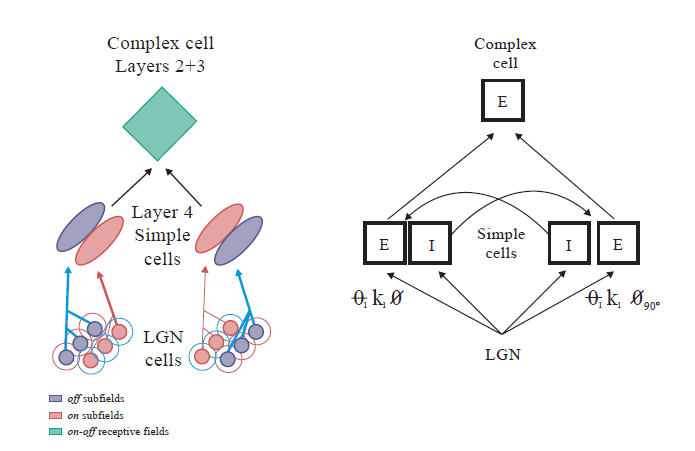
\includegraphics[width=10cm]{figures/models/hierarchical-models.png}
     \caption{Illustration of the hierarchical models (\cite{martinez_complex_2003})}
\end{figure}

\par The possible advantages of hierarchical models are as follows:
\begin{itemize}
    \item If a visual recognition task can be decomposed into low-complexity learning tasks for each layer of a hierarchical learning machine, then each layer may require only a small number of training examples (\cite{poggio2003mathematics}).
    \item The lowest levels of the hierarchy may represent a dictionary of features that can be shared across multiple classification tasks (\cite{geman1999hierarchy}), thus increasing efficiency.
\end{itemize}

\par There are also some known limitations of hierarchical models:
\begin{itemize}
    \item Hierarchical models assume that the computations at each successive stage being largely feed-forward (\cite{riesenhuber1999hierarchical}, \cite{dicarlo2012does}). This is limited because back-projections are also likely to be a key part of the visual system. 
    \item There remains a very broad distribution of tuning and receptive field sizes in all areas of the visual hierarchy. Hence, the anatomical hierarchy should be taken as an idealization and cannot be taken as a strict flowchart of visual information (\cite{hegde2007reappraising}). 
    % \par One particularly interesting piece of evidence: a close comparison of shape representation between V1, V2 and V4 also demonstrated a complex pattern of shape selectivity with significant deviation from strict hierarchical organization with some cells in V1 exhibiting more complex tuning than some cells in V4 (\cite{hegde2007reappraising}).
\end{itemize}

\subsection{Alternative Models}
\par Since Hubel and Wiesel proposed the classification of simple cells and complex cells, many other hierarchical models have been proposed for a more realistic representation for the cortical circuitry. Furthermore, new experimental and computational evidence provided serious alternatives to this hierarchical model, including parallel models and recurrent models (\cite{martinez_complex_2003}). There are still many controversies and debates over which models best capture neural mechanisms of the visual system.

\subsubsection{Parallel Models}
\par The first strong evidence against the hierarchical model was the discovery that some complex cells, like simple cells, receive monosynaptic input from the thalamus (\cite{hoffmann1972relay}). Based on this discovery, Hoffman and Stone proposed that both cell types, simple and complex, were generated in parallel by separate thalamocortical pathways, as shown in diagram A in Figure \ref{fig:parallel-models}. 
\begin{figure}[H]
\centering
    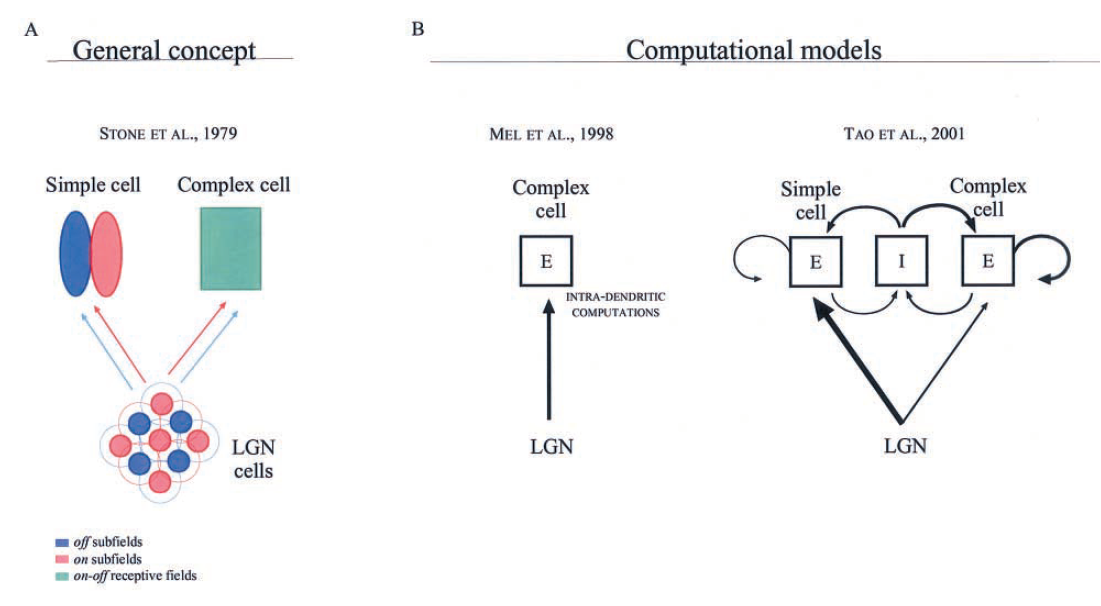
\includegraphics[width=10cm]{figures/models/parallel-models.png}
     \caption{Illustration of the parallel models (\cite{martinez_complex_2003})}
     \label{fig:parallel-models}
\end{figure}

\par Simple cells and complex cells are far from being two parallel cortical pathways in the same way that X and Y cells are parallel thalamic pathways. However, the idea that some complex receptive fields can be generated at
least in part by direct thalamic inputs is likely to be correct. (\cite{martinez_complex_2003})

\subsubsection{Recurrent Models}
\par Recurrent models changed the focus of attention from single cells to networks of cortical connections. (\cite{martinez_complex_2003}) An illustration for recurrent models are shown in Figure \ref{fig:recurrent-models}.

\begin{figure}[H]
\centering
    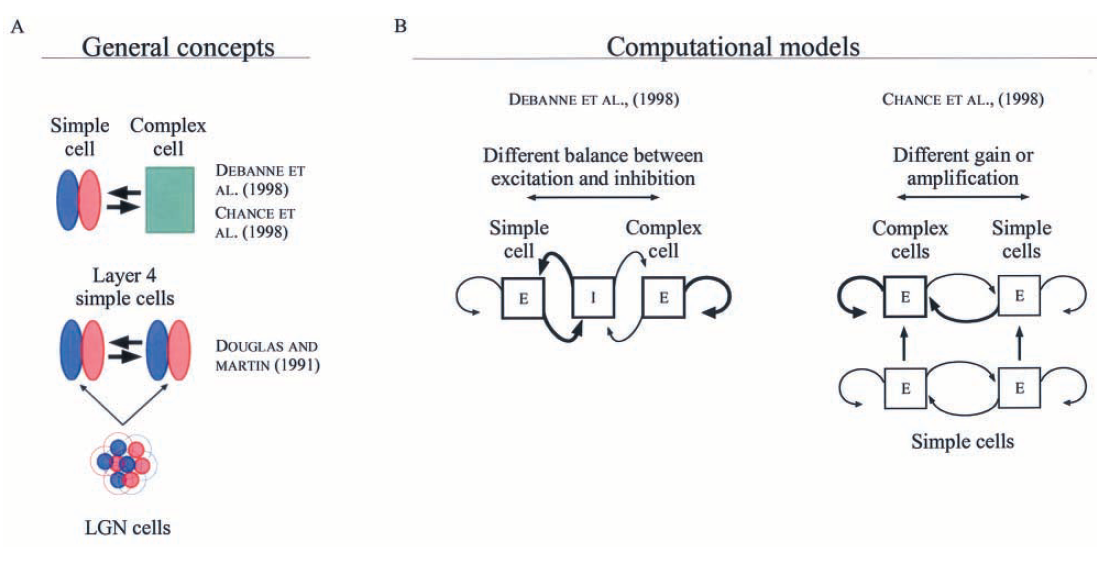
\includegraphics[width=10cm]{figures/models/recurrent-models.png}
     \caption{Illustration of the recurrent models (\cite{martinez_complex_2003})}
     \label{fig:recurrent-models}
\end{figure}

\section{Related works on geometric and topological approach to neural networks}
Throughout the historical progress in neuroscience, there have been numerous efforts to apply geometric and topological methods from related fields in mathematics and computer science, including computational geometry, differential geometry, spectral graph theory, and algebraic topology, among many others. Recently, studying the structure of neural population response with high-dimensional neural spiking data has become a commonly used technique in studying the structure of brain cortices. The high-dimensional nature of neural spiking data have thus motivated various dimensionality reduction methods, both linear and non-linear. 

The paper (\cite{chung_neural_2021}) provided a comprehensive review of the recent studies that have applied geometric and topological methods to discover the properties of neural population geometry. 
% \cite{chung_classification_2018} proposed the ``object manifold" which

The authors of (\cite{gallego_neural_2017}) were the first to propose the concept of ``neural modes," which are specific patterns of correlated neural activity that span the neural manifolds. They thus proposed a generative model of individual neuronal activity based on the activation of neural modes. The parameters of such model can be obtained using dimensionality reduction methods. \cite{williams_unsupervised_2018} used linear dimensionality reduction method of tensor canonical polyadic (CP) decomposition to discover low-dimensional neural dynamics by extracting three ``tensor factors," which are interconnected, low-dimensional descriptions of neural data.

The first work that applied topological methods in neuroscience is (\cite{singh_top_v1_2008}). The authors applied computational topology to analyze neural population activity in the primary visual cortex and concluded that the topological structure of neural population activity is align with the topological structure of a $2$-sphere both when the cortex is spontaneously active and when evoked by natural images.

Following that, there have been many applications of persistent homology in studying the topological structure of neural population activity across different systems. A notable application is (\cite{chaudhuri_intrinsic_2019}), where the authors applied persistent homology to study the the neural population activity from the post-subiculum and anterodorsal thalamus. They showed that the head direction of mice can be decoded from a one-dimensional ring structure. A recent addition to this line of work was (\cite{beshkov_geodesic-based_2021}). The authors of this paper showed that when using the geodesic distance instead of the Euclidean distance, persistent homology method was able to successfully identify highly non-linear features. They then provided an application using the Neuropixels dataset recorded in mouse visual cortex after stimulation with drifting gratings.

\section{Organization of the report}

\par The current chapter outlined the goals and significance of this project, historical background of the research question, and related works. Chapter 2 will give an overview of the methodology and Chapters 3 and 4 will address the different parts of the methodology in greater details. Chapter 5 and 6 will present the implementation details on the experiments for biological and artificial neural networks, respectively. Chapter 7 is an extension of the method to study the topological features of the manifold structure. Chapter 8 will summarize the tasks and results completed during this semester and provide a blueprint for the next steps.